\chapter{Approach}
\label{chap:approach}
This chapter introduces the distinctive concept of a configurable search engine and outlines the comprehensive software architecture. It thoroughly explores and showcases all the required components for constructing the search engine, along with discussing implementation specifics. This encompasses the pivotal models and classes employed for the components and algorithms.
Furthermore, the chapter delves into the user interface, clarifying how it enhances user experience and facilitates configuring the search engine.

\section{Software Architecture}

Figure 4 provides an overview of the software architecture employed by the search engine. Microservices architecture was used to make scalability easier and also to split the responsibilities of each component. Docker is used to enforce this architectural pattern where the Ubuntu:18.04 image is used for each component. Below is a compilation of the utilized technology stack:

\begin{figure}[h]	
     \centering
     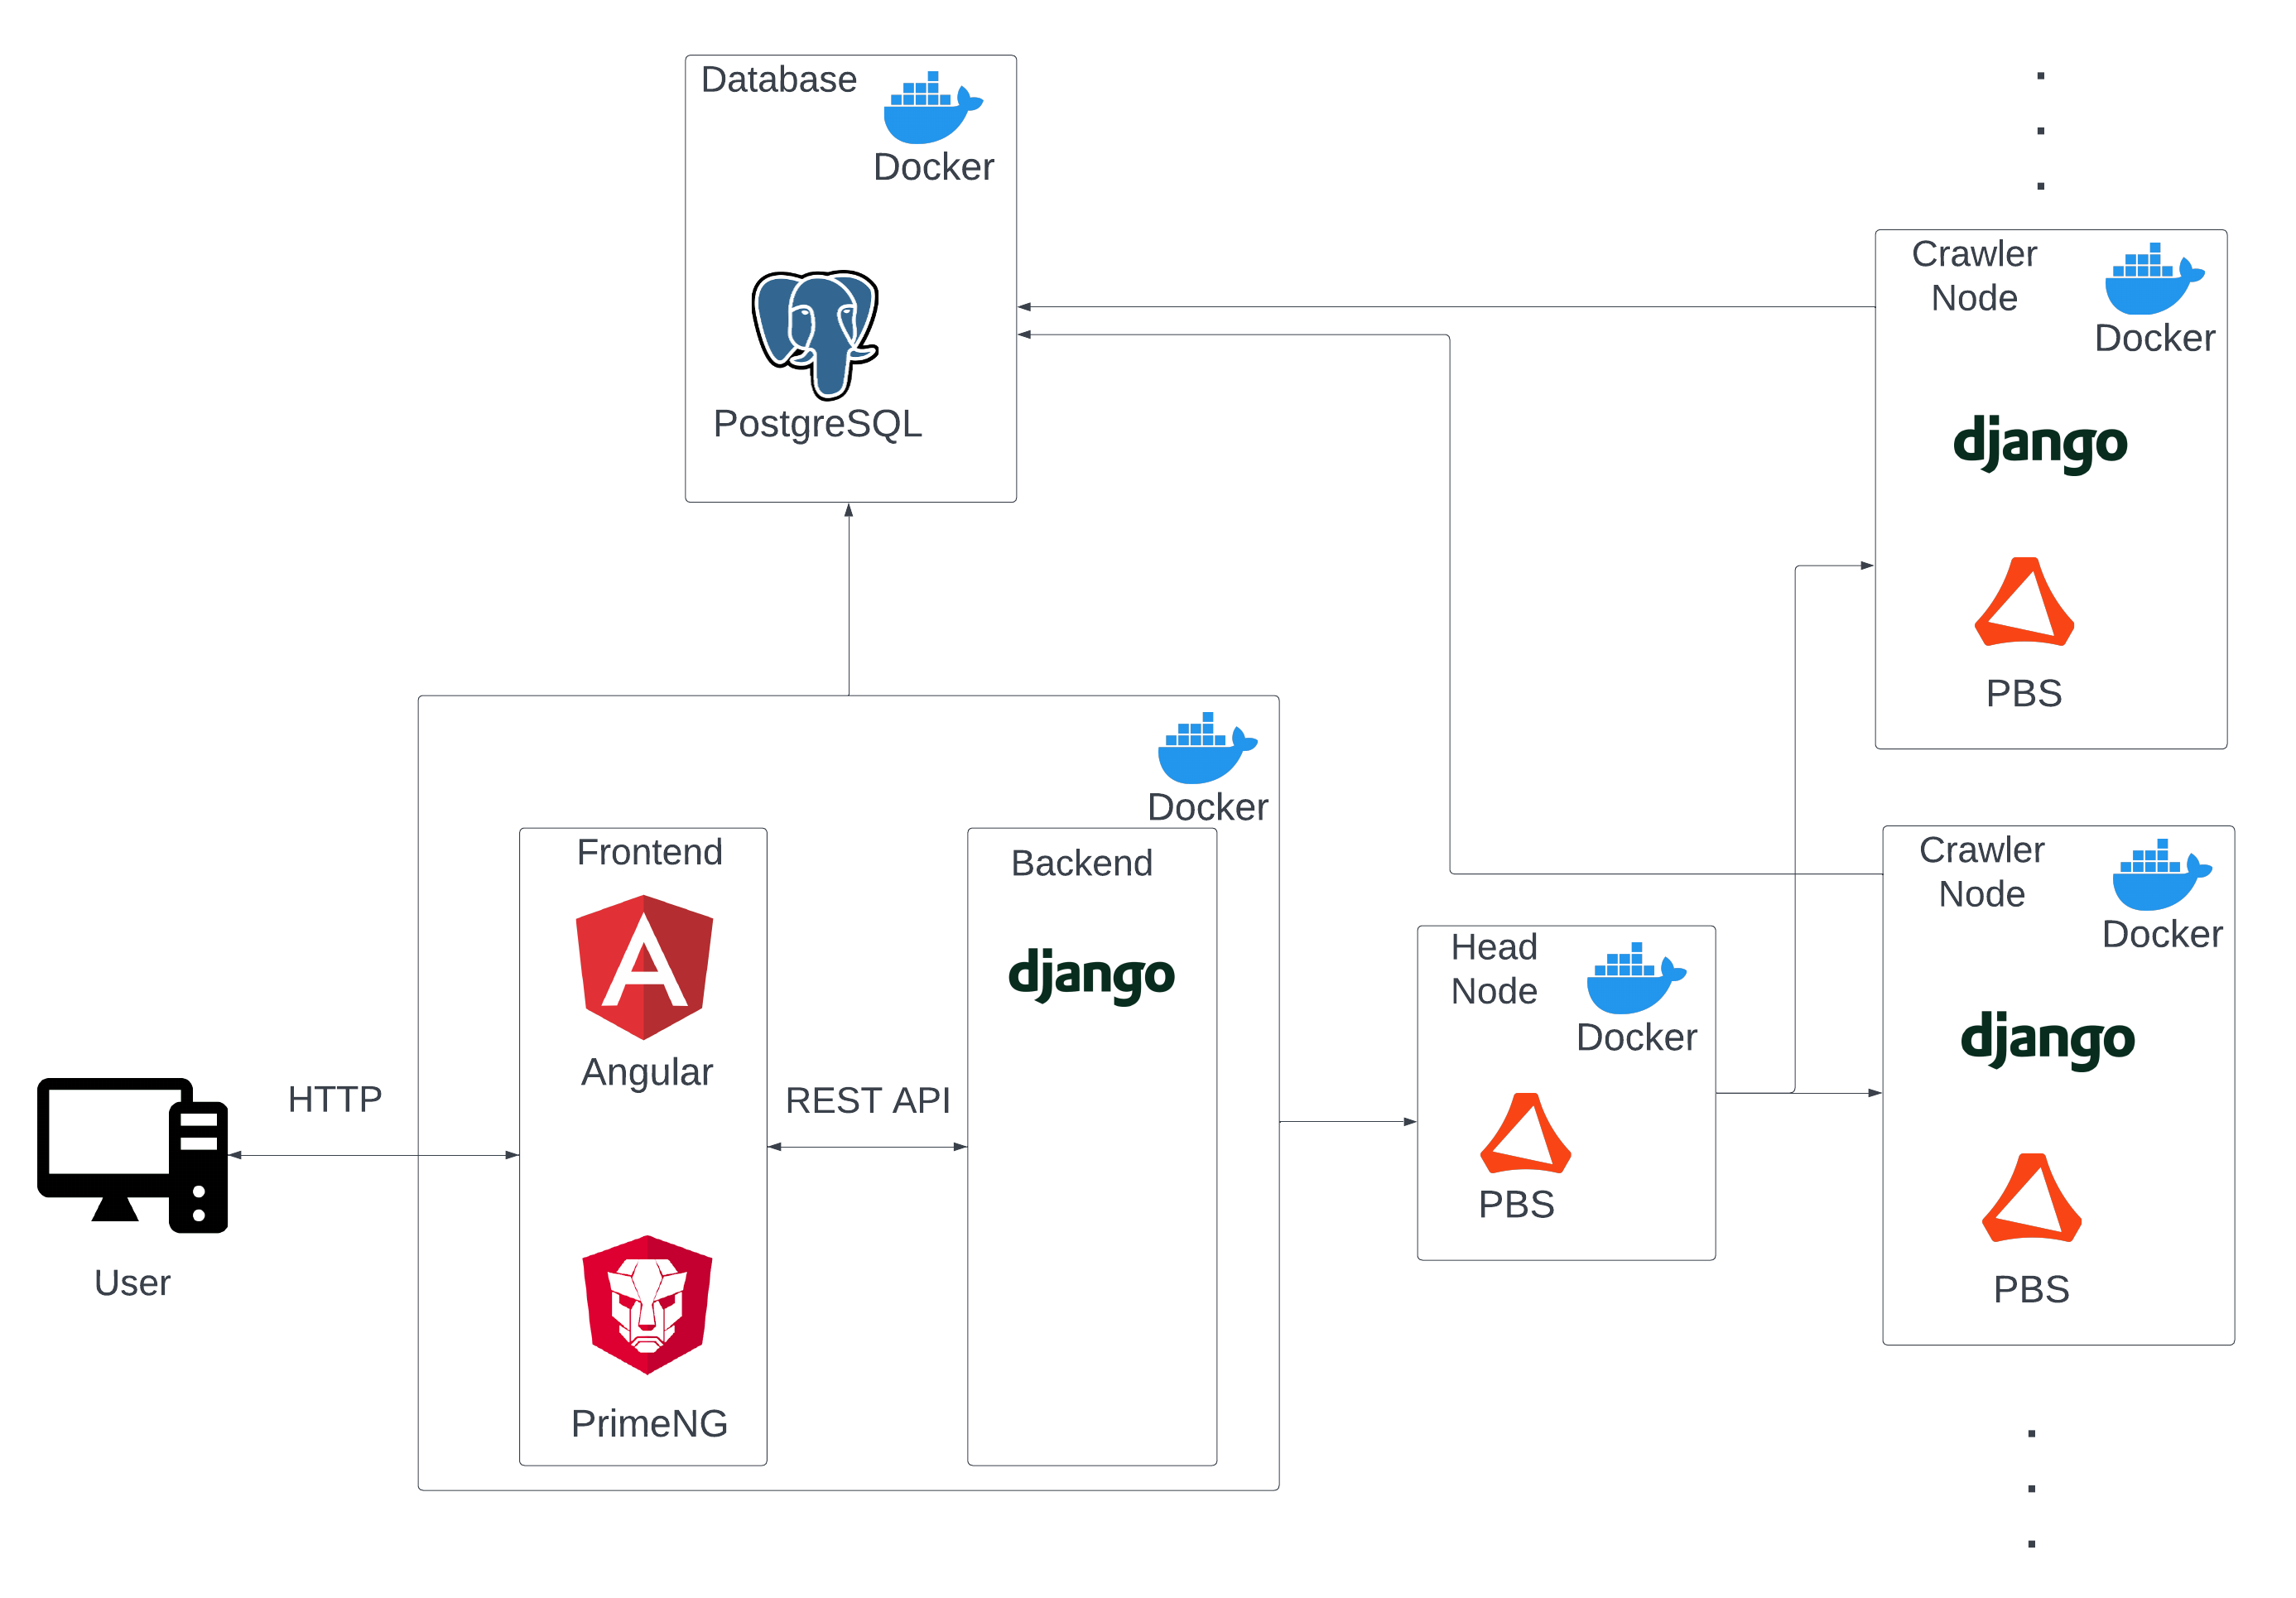
\includegraphics[width=10cm]{images/software_arch.png}
     \caption{High-level view of the software archtiticture.}
     \label{fig:software-arch}
\end{figure}

\begin{itemize}
  \item \textbf{Frontend (Angular \& PrimeNG)}: Positioned closest to the user, this component encompasses all pages and views. Angular is leveraged in conjunction with the contemporary CSS library, PrimeNG. To communicate with the backend, it employs the REST API.
  \item \textbf{Backend (Django)}: Serving as the core intelligence of the search engine, the backend houses both the crawler and indexer modules. It facilitates interaction with the Head node to initiate crawling based on user-defined configurations. Moreover, it establishes a connection with PostgreSQL for the storage of crawler and indexer configurations, along with job-related information.
  \item \textbf{Head Node (PBS)}: Operating as the central hub, this node orchestrates job management and determines the allocation of tasks to Crawler nodes, which are responsible for traversing the specified websites.
  \item \textbf{Crawler Node (PBS)}: These instances are designated to execute the crawling process and store the resulting data in the PostgreSQL database.
\end{itemize}


\subsection{Crawler Implmentation}
\begin{algorithm}[H]
	\caption{$Start Crawling$}\label{alg:alg1}
	\begin{algorithmic}
		\State $thread$ $\gets$ $create\_threads\_pool()$
	    \State $urls\_queue$ $\gets$ $get\_thread\_urls\_queue(thread)$
	    \State $load\_crawler\_configurations()$
	    \State $seed\_url$ $\gets$ $get\_seed\_url()$
	    \State $robot\_file$ $\gets$ $get\_robot\_file\_content()$
	    \State $sdd\_ulr\_to\_queue(urls\_queue, seed\_url)$
	    \While {$urls\_queue$ not empty or All threads not done}
		\If{$urls\_queue$ is empty}
		    \State $urls\_queue$ $\gets$ $get\_thread\_urls\_queue(thread)$
		\Else
			\State $current\_url$ $\gets$ $urls\_queue.pop()$
			\State $filter\_unwanted\_urls(current\_url)$
			\State $content$ $\gets$ $request\_page(current\_url)$
			\State $find\_next\_urls\_and\_add\_them\_to\_urls\_queue()$
			\State $docs$ $\gets$ $find\_and\_download\_targeted\_documents()$
			\State $filter\_unwanted\_documents(docs)$
		\EndIf
		\EndWhile

	\end{algorithmic}
\end{algorithm}

\subsection{Indexer Implmentation}